% -*-cap1.tex-*-
% Este fichero es parte de la plantilla LaTeX para
% la realización de Proyectos Final de Carrera, protejido
% bajo los términos de la licencia GFDL.
% Para más información, la licencia completa viene incluida en el
% fichero fdl-1.3.tex

% Copyright (C) 2009 Pablo Recio Quijano 

%\section{Introducción}

A continuación se muestran los resultados del estudio tal y como se describieron en la sección anterior.

\section{Localización de la literatura}
En la tabla \ref{tab:ResumenBusquedaResultados} se muestran el número de publicaciones devueltas para cada búsqueda por las bibliotecas digitales utilizadas en este estudio. En total se recopilaron 467 trabajos, que fueron revisados para identificar si eran de utilidad para el estudio. 

\begin{table}[H]
  \begin{center}
  \begin{tabular}{| m{3.5cm} | m{6cm} | m{3cm} | c |}
    \hline
    SOURCE & SEARCH TERMS & SEARCH SCOPE & RESULTS\\
    \hline
    \hline
    Wiley Online Library & assessment AND ``generic competences`` OR ``generic skills`` AND (TEL OR ICT OR CBI) & in All Fields & 140 \\
    \hline
    World Scientific Net & ``generic competences`` OR ``generic skills`` AND assessment & Anywhere in article & 20\\
    \hline
    Springer & (``generic skills`` OR ``generic competences``) AND  students AND (TEL OR CBI OR ICT) & All fields (Including full text) & 140\\
    \hline
    ACM Digital Library & (assessment and ``generic skills``) and (TEL or LMS or ICT or CBI) & Any field (title, abstract, review) & 57\\
    \hline
    ACM Digital Library & (assessment and ``generic competences``) and (TEL or LMS or ICT or CBI) & Any field (title, abstract, review) & 15\\
    \hline
    IEEE Digital Library (Xplore) & (((TEL or LMS or ICT or CBI) AND (``generic skills`` OR ``generic competences``)) AND assessment) & Full text and metadata & 48\\
    \hline
    Scopus & (((TEL or LMS or ICT or CBI) AND (``generic skills`` OR ``generic competences``)) AND assessment) & All fields (Including full text) & 47\\
    \hline
    \multicolumn{3}{|r|}{TOTAL} & 467\\
    \hline
  \end{tabular}
\end{center}
\caption{Resumen de búsqueda de bibliografía}
\label{tab:ResumenBusquedaResultados}
\end{table} 


\section{Selección de trabajos}
En la tabla \ref{tab:ResumenSelecccionResultados} se muestran los resultados de la clasificación.

\begin{table}[H]
  \begin{center}
  \begin{tabular}{| m{4cm} | c | c |}
    \hline
    CRITERION & STUDIES & FRECUENCY\\
    \hline
    \hline 
    Included & 64 & 13,70\% \\
    \hline
    Off Topic & 374 & 80,09\% \\
    \hline
    Unsupported Language & 1 & 0,21\% \\
    \hline
    Out Scope & 2 & 0,43\% \\
    \hline
    Duplicated & 20 & 4,28\% \\
    \hline
    Unread & 6 & 1,28\% \\
    \hline
    Total & 467 & 100\% \\
    \hline
  \end{tabular}
\end{center}
\caption{Resumen de selección de bibliografía}
\label{tab:ResumenSelecccionResultados}
\end{table} 


\section{Extracción de los datos}
Se han seleccionado como estudio primario únicamente 64 artículos, un 13,7\% del total de los revisados. Casi la mayor parte de los seleccionados se pueden localizar en los últimos años, entre 2008 y 2013 (Tabla \ref{tab:ResumenAniosResultados} y figura \ref{fig:PublicacionesAnuales}). Siendo las revistas el medio en el que más de este tipo de artículos se han publicado, tal y como se puede consultar en la tabla \ref{tab:ResumenForumResultados} y en la figura \ref{fig:PublicacionesForum}.


\begin{table}[H]
  \begin{center}
  \begin{tabular}{| m{4cm} | c |}
    \hline
    YEAR & RESULTS\\
    \hline
    \hline 
    1996 & 1\\
    \hline
    1997 & 1\\
    \hline
    1998 & 0\\
    \hline
    1999 & 1\\
    \hline
    2000 & 0\\
    \hline
    2001 & 0\\
    \hline
    2002 & 0\\
    \hline
    2003 & 1\\
    \hline
    2004 & 1\\
    \hline
    2005 & 2\\
    \hline
    2006 & 2\\
    \hline
    2007 & 4\\
    \hline
    2008 & 13\\
    \hline
    2009 & 4\\
    \hline
    2010 & 5\\
    \hline
    2011 & 6\\
    \hline
    2012 & 8\\
    \hline
    2013 & 14 \\
    \hline
  \end{tabular}
\end{center}
\caption{Resumen de selección de bibliografía}
\label{tab:ResumenAniosResultados}
\end{table} 

\begin{figure}[H]
  \begin{center}
    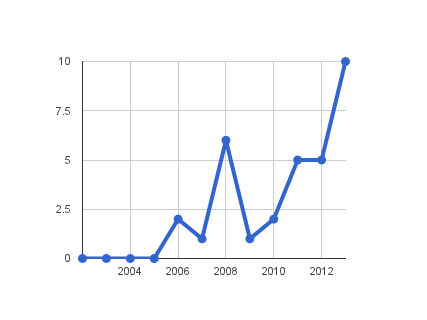
\includegraphics[scale=0.8]{cap3_pub_anuales.png}
  \end{center}
  \caption{Distribución de publicaciones por años}
  \label{fig:PublicacionesAnuales}
\end{figure}

\begin{table}[H]
  \begin{center}
  \begin{tabular}{| m{4cm} | c |}
    \hline
    PUBLICATION FORUM & RESULTS\\
    \hline
    \hline 
    Journal & 36 \\
    \hline
    Conference & 15 \\
    \hline
    Chapter & 11 \\
    \hline
  \end{tabular}
\end{center}
\caption{Resumen de selección de bibliografía}
\label{tab:ResumenForumResultados}
\end{table} 

\begin{figure}[H]
  \begin{center}
    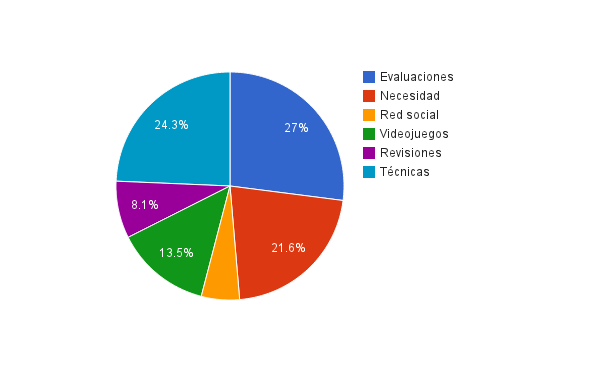
\includegraphics[scale=0.8]{cap3_pub_forum.png}
  \end{center}
  \caption{Distribución de publicaciones por soporte}
  \label{fig:PublicacionesForum}
\end{figure}



\section{Análisis y síntesis de los datos}

....
